\documentclass{article}
\usepackage{amsmath}
\usepackage{graphicx}
\usepackage{tikz}
\usetikzlibrary{arrows.meta,positioning}
% To paste into another document: copy the two figure environments below and
% add graphicx, tikz and \usetikzlibrary{arrows.meta,positioning} to its preamble.
\begin{document}

\begin{figure}[htbp]
\centering
\resizebox{0.75\textwidth}{!}{%
\begin{tabular}{c@{\hskip 1.4cm}c}
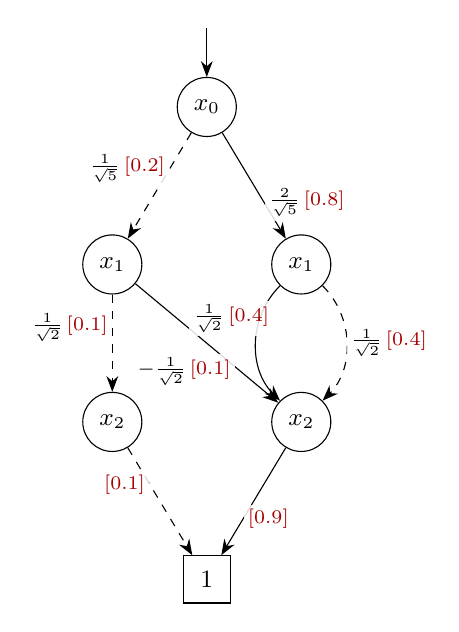
\begin{tikzpicture}[
    every node/.style={font=\small},
    nd/.style={circle, draw, minimum size=7.5mm, inner sep=0pt},
    tm/.style={rectangle, draw, minimum size=6mm, inner sep=2pt},
    e/.style={-{Stealth[length=2mm]}},
    lbl/.style={font=\scriptsize, inner sep=1.5pt, fill=white,
                fill opacity=0.85, text opacity=1},
    idl/.style={font=\tiny, inner sep=1pt, gray},
  ]
  \node[nd] (n5) at (0.00, 0.00) {$x_{0}$};
  \node[nd] (n3) at (-1.20, -2.00) {$x_{1}$};
  \node[nd] (n4) at (1.20, -2.00) {$x_{1}$};
  \node[nd] (n1) at (-1.20, -4.00) {$x_{2}$};
  \node[nd] (n2) at (1.20, -4.00) {$x_{2}$};
  \node[tm] (term) at (0, -6.00) {$1$};
  \coordinate (in) at (0.00, 1.00);
  \draw[e] (in) -- (n5);
  \draw[e, dashed] (n1) -- node[lbl, left, pos=0.34] {{\color{red!65!black}[0.1]}} (term);
  \draw[e, solid] (n2) -- node[lbl, right, pos=0.66] {{\color{red!65!black}[0.9]}} (term);
  \draw[e, dashed] (n3) -- node[lbl, left, pos=0.34] {$\tfrac{1}{\sqrt{2}}$\,{\color{red!65!black}[0.1]}} (n1);
  \draw[e, solid] (n3) -- node[lbl, below left, pos=0.7, yshift=5pt] {$-\tfrac{1}{\sqrt{2}}$\,{\color{red!65!black}[0.1]}} (n2);
  \draw[e, dashed] (n4) to[bend left=45] node[lbl, right, pos=0.5] {$\tfrac{1}{\sqrt{2}}$\,{\color{red!65!black}[0.4]}} (n2);
  \draw[e, solid] (n4) to[bend right=45] node[lbl, left, pos=0.3, xshift=5pt] {$\tfrac{1}{\sqrt{2}}$\,{\color{red!65!black}[0.4]}} (n2);
  \draw[e, dashed] (n5) -- node[lbl, left, pos=0.34] {$\tfrac{1}{\sqrt{5}}$\,{\color{red!65!black}[0.2]}} (n3);
  \draw[e, solid] (n5) -- node[lbl, right, pos=0.66] {$\tfrac{2}{\sqrt{5}}$\,{\color{red!65!black}[0.8]}} (n4);
\end{tikzpicture}
&
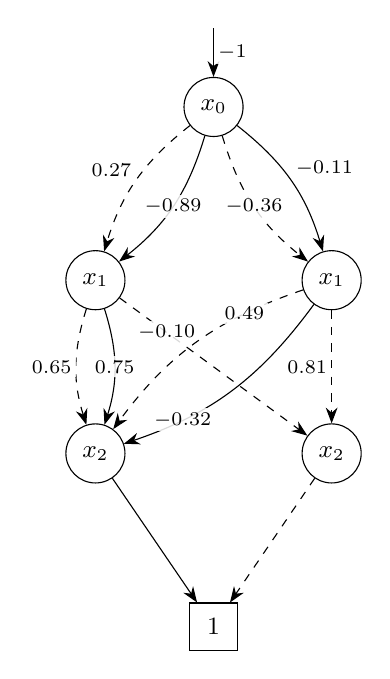
\begin{tikzpicture}[
    every node/.style={font=\small},
    nd/.style={circle, draw, minimum size=7.5mm, inner sep=0pt},
    tm/.style={rectangle, draw, minimum size=6mm, inner sep=2pt},
    e/.style={-{Stealth[length=2mm]}},
    lbl/.style={font=\scriptsize, inner sep=1.5pt, fill=white,
                fill opacity=0.85, text opacity=1},
    idl/.style={font=\tiny, inner sep=1pt, gray},
  ]
  \node[nd] (n5) at (0.00, 0.00) {$x_{0}$};
  \node[nd] (n3) at (-1.50, -2.20) {$x_{1}$};
  \node[nd] (n4) at (1.50, -2.20) {$x_{1}$};
  \node[nd] (n1) at (-1.50, -4.40) {$x_{2}$};
  \node[nd] (n2) at (1.50, -4.40) {$x_{2}$};
  \node[tm] (term) at (0, -6.60) {$1$};
  \coordinate (in) at (0.00, 1.00);
  \draw[e, solid] (in) -- node[lbl, right] {$-1$} (n5);
  \draw[e, dashed] (n5) to[bend right=17.5] node[lbl, auto, swap, pos=0.5] {$0.27$} (n3);
  \draw[e, solid] (n5) to[bend left=17.5] node[lbl, pos=0.5] {$-0.89$} (n3);
  \draw[e, dashed] (n5) to[bend right=17.5] node[lbl, pos=0.5] {$-0.36$} (n4);
  \draw[e, solid] (n5) to[bend left=17.5] node[lbl, auto, pos=0.5] {$-0.11$} (n4);
  \draw[e, dashed] (n3) to[bend right=17.5] node[lbl, auto, swap, pos=0.5] {$0.65$} (n1);
  \draw[e, solid] (n3) to[bend left=17.5] node[lbl, pos=0.5] {$0.75$} (n1);
  \draw[e, dashed] (n3) -- node[lbl, pos=0.25] {$-0.10$} (n2);
  \draw[e, dashed] (n4) to[bend right=17.5] node[lbl, pos=0.25] {$0.49$} (n1);
  \draw[e, solid] (n4) to[bend left=17.5] node[lbl, pos=0.75] {$-0.32$} (n1);
  \draw[e, dashed] (n4) -- node[lbl, left, pos=0.5] {$0.81$} (n2);
  \draw[e, solid] (n1) -- (term);
  \draw[e, dashed] (n2) -- (term);
\end{tikzpicture}
\\[4pt] exact: 5 nodes & exact nd-EVDD from TT (non-deterministic): 5 nodes, 12 edges
\end{tabular}%
}
\caption{State of Fig.~1(a) in Hillmich et al.: exact EVDD, with the norm
contribution of every edge in brackets, and the nd-EVDD of the untruncated TT.}
\end{figure}

\begin{figure}[htbp]
\centering
\resizebox{\textwidth}{!}{%
\begin{tabular}{c@{\hskip 1.4cm}c@{\hskip 1.4cm}c}
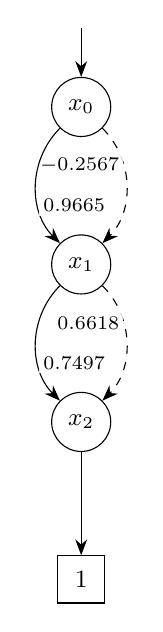
\begin{tikzpicture}[
    every node/.style={font=\small},
    nd/.style={circle, draw, minimum size=7.5mm, inner sep=0pt},
    tm/.style={rectangle, draw, minimum size=6mm, inner sep=2pt},
    e/.style={-{Stealth[length=2mm]}},
    lbl/.style={font=\scriptsize, inner sep=1.5pt, fill=white,
                fill opacity=0.85, text opacity=1},
    idl/.style={font=\tiny, inner sep=1pt, gray},
  ]
  \node[nd] (n3) at (0.00, 0.00) {$x_{0}$};
  \node[nd] (n2) at (0.00, -2.00) {$x_{1}$};
  \node[nd] (n1) at (0.00, -4.00) {$x_{2}$};
  \node[tm] (term) at (0, -6.00) {$1$};
  \coordinate (in) at (0.00, 1.00);
  \draw[e] (in) -- (n3);
  \draw[e, solid] (n1) -- (term);
  \draw[e, dashed] (n2) to[bend left=45] node[lbl, left, pos=0.34] {$0.6618$} (n1);
  \draw[e, solid] (n2) to[bend right=45] node[lbl, right, pos=0.66] {$0.7497$} (n1);
  \draw[e, dashed] (n3) to[bend left=45] node[lbl, left, pos=0.34] {$-0.2567$} (n2);
  \draw[e, solid] (n3) to[bend right=45] node[lbl, right, pos=0.66] {$0.9665$} (n2);
\end{tikzpicture}
&
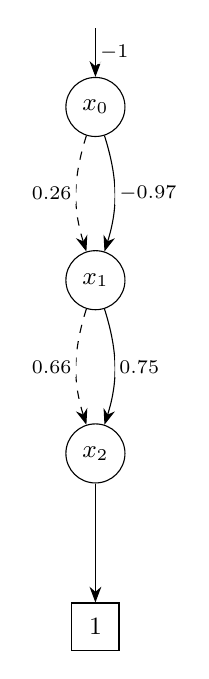
\begin{tikzpicture}[
    every node/.style={font=\small},
    nd/.style={circle, draw, minimum size=7.5mm, inner sep=0pt},
    tm/.style={rectangle, draw, minimum size=6mm, inner sep=2pt},
    e/.style={-{Stealth[length=2mm]}},
    lbl/.style={font=\scriptsize, inner sep=1.5pt, fill=white,
                fill opacity=0.85, text opacity=1},
    idl/.style={font=\tiny, inner sep=1pt, gray},
  ]
  \node[nd] (n3) at (0.00, 0.00) {$x_{0}$};
  \node[nd] (n2) at (0.00, -2.20) {$x_{1}$};
  \node[nd] (n1) at (0.00, -4.40) {$x_{2}$};
  \node[tm] (term) at (0, -6.60) {$1$};
  \coordinate (in) at (0.00, 1.00);
  \draw[e, solid] (in) -- node[lbl, right] {$-1$} (n3);
  \draw[e, dashed] (n3) to[bend right=17.5] node[lbl, auto, swap, pos=0.5] {$0.26$} (n2);
  \draw[e, solid] (n3) to[bend left=17.5] node[lbl, auto, pos=0.5] {$-0.97$} (n2);
  \draw[e, dashed] (n2) to[bend right=17.5] node[lbl, auto, swap, pos=0.5] {$0.66$} (n1);
  \draw[e, solid] (n2) to[bend left=17.5] node[lbl, auto, pos=0.5] {$0.75$} (n1);
  \draw[e, solid] (n1) -- (term);
\end{tikzpicture}
&
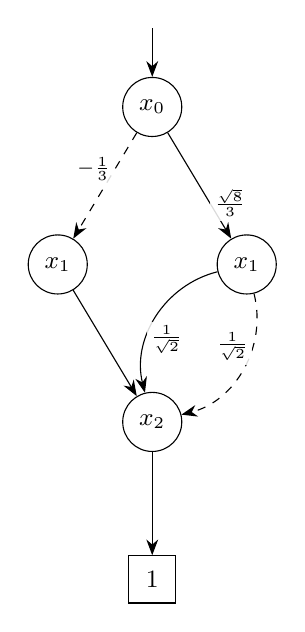
\begin{tikzpicture}[
    every node/.style={font=\small},
    nd/.style={circle, draw, minimum size=7.5mm, inner sep=0pt},
    tm/.style={rectangle, draw, minimum size=6mm, inner sep=2pt},
    e/.style={-{Stealth[length=2mm]}},
    lbl/.style={font=\scriptsize, inner sep=1.5pt, fill=white,
                fill opacity=0.85, text opacity=1},
    idl/.style={font=\tiny, inner sep=1pt, gray},
  ]
  \node[nd] (n7) at (0.00, 0.00) {$x_{0}$};
  \node[nd] (n6) at (-1.20, -2.00) {$x_{1}$};
  \node[nd] (n4) at (1.20, -2.00) {$x_{1}$};
  \node[nd] (n2) at (0.00, -4.00) {$x_{2}$};
  \node[tm] (term) at (0, -6.00) {$1$};
  \coordinate (in) at (0.00, 1.00);
  \draw[e] (in) -- (n7);
  \draw[e, solid] (n2) -- (term);
  \draw[e, dashed] (n4) to[bend left=45] node[lbl, left, pos=0.34] {$\tfrac{1}{\sqrt{2}}$} (n2);
  \draw[e, solid] (n4) to[bend right=45] node[lbl, right, pos=0.66] {$\tfrac{1}{\sqrt{2}}$} (n2);
  \draw[e, solid] (n6) -- (n2);
  \draw[e, dashed] (n7) -- node[lbl, left, pos=0.34] {$-\tfrac{1}{3}$} (n6);
  \draw[e, solid] (n7) -- node[lbl, right, pos=0.66] {$\tfrac{\sqrt{8}}{3}$} (n4);
\end{tikzpicture}
\\[4pt] $\chi=1$, TT $\to$ det: 3 nodes, $F=0.853$ & nd-EVDD from TT: 3 nodes, 5 edges & Hillmich $f=0.853$: 4 nodes, $F=0.900$
\end{tabular}%
}
\caption{Truncation to $\chi=1$: the deterministic EVDD obtained from the
truncated TT, the nd-EVDD it comes from, and the Hillmich approximation at the
same fidelity.}
\end{figure}

\end{document}
